\section*{Задание 1}

\subsection*{Задание}

Найдите радиус, диаметр и центр данного дерева (рис \ref{fig:1t}).

\begin{figure}[H]
    \centering
    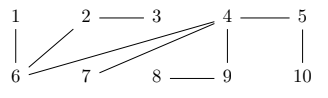
\includegraphics[width=0.7\linewidth]{photo/1t}
    \caption{}
    \label{fig:1t}
\end{figure}

\subsection*{Решение}

\underline{Центр графа}: Вершина \textit{4} или Вершина \textit{6}

Для обоих вершин максимальное расстояние между ними
и любой другой вершиной является 
наименьшим из всех возможных --- 3.

\underline{Радиус графа}: \textbf{3}

$(4 \rightarrow 6 \rightarrow 2 \rightarrow 3)$ 
или
$(6 \rightarrow 4 \rightarrow 8 \rightarrow 9)$ 
или
$(6 \rightarrow 4 \rightarrow 5 \rightarrow 10)$.

\underline{Диаметр графа}: \textbf{5}

$(3 \rightarrow 2 \rightarrow 6 \rightarrow 4 \rightarrow 9 \rightarrow 8)$ 
или
$(3 \rightarrow 2 \rightarrow 6 \rightarrow 4 \rightarrow 5 \rightarrow 10)$.
